The fabrication of a functioning field effect structure of \tmdg mono- or bilayers roughly consists of three different procedures. The production of suitible flakes of \tmd's, the preparation of an electrode both on the sample and in the substrate and the assembly of the full device on top of it. 

\section{Mechanical exfoliation}
\begin{figure}
\centering
\begin{subfigure}{0.4\textwidth}
	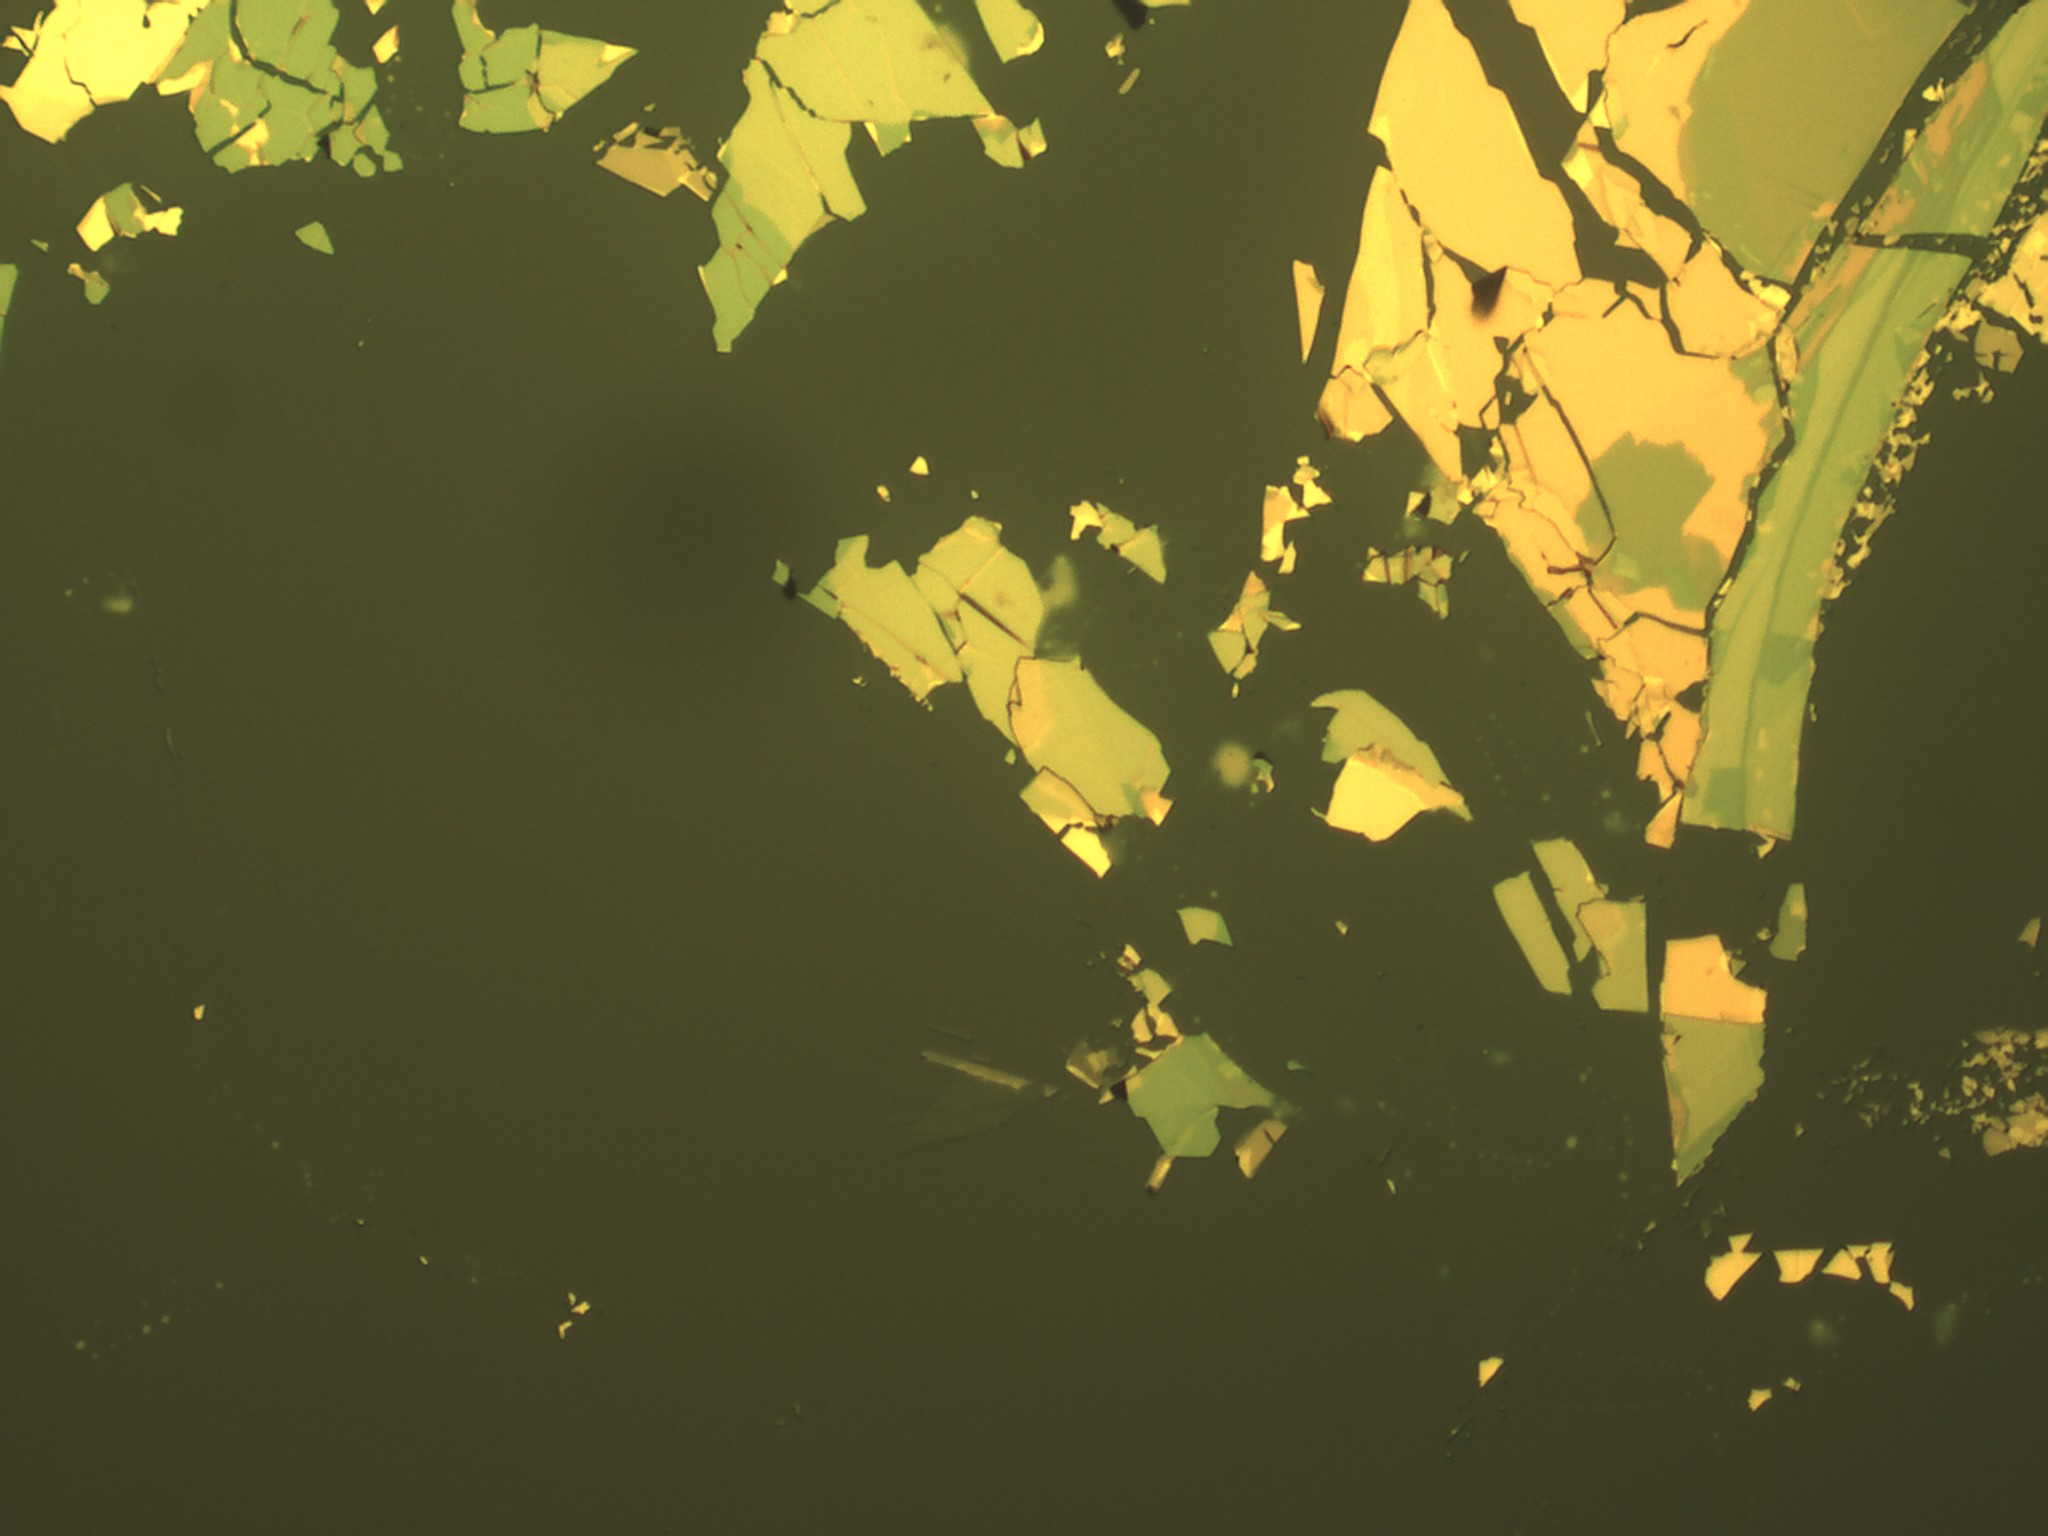
\includegraphics[width=\textwidth]{flakes.jpg}
\end{subfigure}
\begin{subfigure}{0.349\textwidth}
	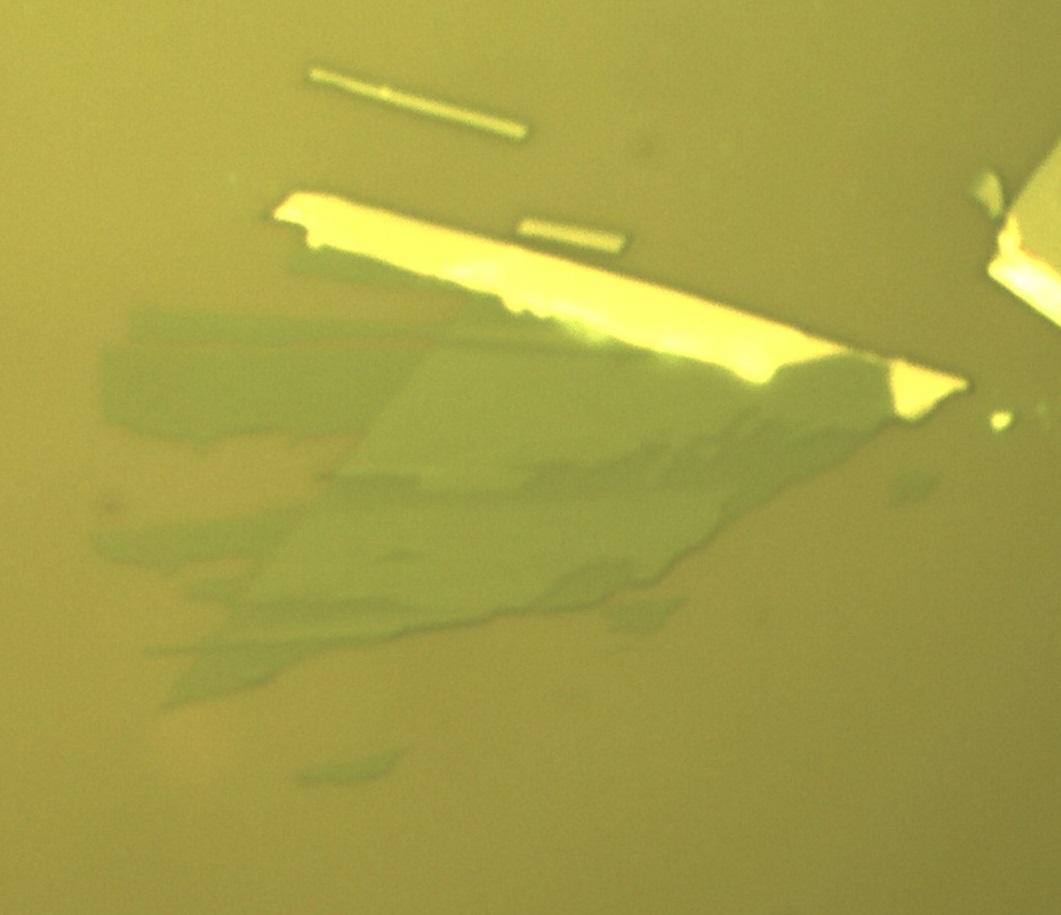
\includegraphics[width=\textwidth]{mono_on_sio2.jpg}
\end{subfigure}
\caption{\textbf{Left:} During the exfoliation process a lot of flakes of different size and thickness are scattered over the substrate. Interesting specimen have to be searched for by hand. \textbf{Right:} Flake consting of mono- and bilayer regions that can be identified by their optical contrast.}
	\label{flakes}
\end{figure}
Thin films of layered materials like \tmd's, like many natomaterials, can be fabricated using a top-down or bottom-up approach. The bottom-up approach for these particular materials is called chemical-vapor deposition (CVD) (Reference). Because of its scalability it is the leading candidate that could be used in an industrial fabrication pipeline. However, the top-down approach of mechanical exfoliatioin (Refernence) has become the first choice for a lot of projects to build high quality model systems, that can be used to study physics in low dimensions. The reason is the so far supperior quality of few-layer flakes in terms of defects and contaminants as well as the synergy with dry transfer methods(Reference(Laterchapter)). 

The mechanical exfoliation process -- oftern referred to as the ``scotch tape method'' -- is based on the fact, that the van-der-Waals forces between adjacent layers in \tmd's are much weaker, than the lateral covalent bonds inside them. In fact, they are weak enough, that they can be easily broken appart by adhesive tape.

The starting point is a solid crystal of \tmd-material, that can be produced either naturally or synthetically with high purity (supplied by hq-graphene). When a stripe of adhesive tape is brought in contact with it, a small amount can be peeled off. With a second stripe, that is put on the first one, the process is repeated multiple times. Each time, the fresh tape is peeled of its parent, the strong adhesion between tape and \tmdg ensures a clean interface. Three to four repetitions are an optimum to produce monolayers of a useful size. More repetitions further thin the material but heighten the risk of these thin films to break to smaller peaces, which complicates processing the flakes later on and build larger devices. 

To prepare monolayer flakes for the assembly of more complex devices, they first have to be transferred onto a suitible substrate. In this work, this substrate is silicon with a layer of thermal oxide that is between 50 and 90 nm thick. Before wafers of this material are brought in contact with the exfoliation tapes they are cleaned both in acetone and isopropanole before being exposed to oxygen plasma for 180 s. This ensures a clean surface and maximizes the material that sticks to the wafer(Reference). After the tape is in contact, the wafer is heated to 90°C. After cooling down the tape can be peeled off and the wafer is inspected for monolayers. As seen in [Figure], during this process a large number of flakes of different sizes and thicknesses are transferred and it is uncommon to find more than one monolayer of suitible size on a wafer of 10 by 10 mm. 

\subsection{Layer number}

\begin{figure}
	\centering
	\begin{subfigure}{0.4\textwidth}
	\adjincludegraphics[trim={0 0 0 0}, width=\textwidth, clip]{Monolayer_Microscope.png}
	\end{subfigure}
	\begin{subfigure}{0.4\textwidth}
	\adjincludegraphics[trim={0 0 0 0}, width=\textwidth, clip]{other_mono_bi_PL.png}
	\end{subfigure}
	\caption{Comparison of mono- and bilayers of WSe$_2$. \textbf{a} The reflectance contrast of mono- and bilayers can be used to measure the layer number. The difference is however small enough to misidentify them under changing or inhomogenious lighting conditions. \textbf{b} The monolayer shows much higher \textsc{pl}-intensity than the bilayer and can therefore be identified very easily.}
	\label{pl-contrast}
\end{figure}

Under an optical microscope monolayers can be identified using the optical contrast and the color. It is possible to verify the layer number by this criteria alone using a camera and image analysis software(Reference/Victor?), however this is much more reliable on transparent substrates, since the optical contrast is higher and the lighting conditions can be controlled more precisely. With our optical microscope and \si/\sio substrates, monolayer candidates where instead verified using photoluminescence (\textsc{pl}) imaging(Referenz Andre). Because of the direct band-gap, monolayers of \tmd's are much more efficient emitters than even bilayers with almost an order of magnitude difference in \textsc{pl}-intesity. The result can be seen in Figure \ref{pl-contrast}. The sample is excited with a laser with a wavelength above the A-exciton resonance and only the \textsc{pl} is collected on the chip of a \textsc{usb}-camera. A detailled description of the optical setup can be found in (Optical Setup). As can be seen, the \textsc{pl}-image clearly identifies the monolayer-regions through bright intensity, while the bilayer region of the flake is not visible at all. On the microscope picture on the other hand, both regions do not differ much in color and reflectance and can be tricky to tell appart, especially when the lighting is inhomogenious or changes over time.

Other methods to idetify monolayers inlcude both photoluminescence and Raman spectroscopy(Reference). However, for assembling devices and verifying the quality of exfoliated flakes, \textsc{pl}-imaging proved to be the fastest and most versatile method.

\section{Hexagonal boron nitride}

For spectroscopic studies of \tmd's the right substrate plays one of the most crucial parts. Hexagonal boron nitride (\hbn) has proven to be the supperior choice to observe narrow linewith spectra in \tmd's. On substrates like \sio dangling bonds and strain due to surface roughness can induce scattering of excitons, that reduce the lifetime and induce inhomogenious broadening. This effects are strong enough make many different spectral features indistinguishible. \hbn is an has a large indirect band-gap in the \textsc{uv}-range, and acts like a transparent insulator. Furthermore, its graphene-like crystal structure allows the exfoliation of atomically flat terasses, that can be used as a dielectrically calm substrate, not only for optical measurements on \tmds but for other areas of layered materials as well. The best results have been obtained by not only placing flakes on \hbn but to fully incapsulate them. Since \hbn, much like \tmds is a layered material, flakes of it can be exfoliated in the same manner and \tmd-monolayers can be fully encapsulated by ``sandwitching'' them between two flakes of \hbn.

\section{Electrode fabrication}

The goal of this thesis was, to fabricate high quality \tmd-monolayer samples that are gate-tunable, meaning control over the charge density inside the monolayer flake leveraging the field effect. The problem of designing such a device can be understood as using the 2D-material as one plate of a capacitor, and charging it, by applying a voltage. The other plate or ``back-gate'' in this analogy is the conducting boron-doped silicon substrate. Flake and substrate are separated by a 50nm layer of thermal silicon-dioxide, that functions as the dielectric of the gate-structure. Both the sample on top and the back-gate have to be contacted to allow the application of a voltage.

\subsection{uv-lithography}

\begin{figure}
\centering
\begin{subfigure}{0.4\textwidth}
	\caption{}
	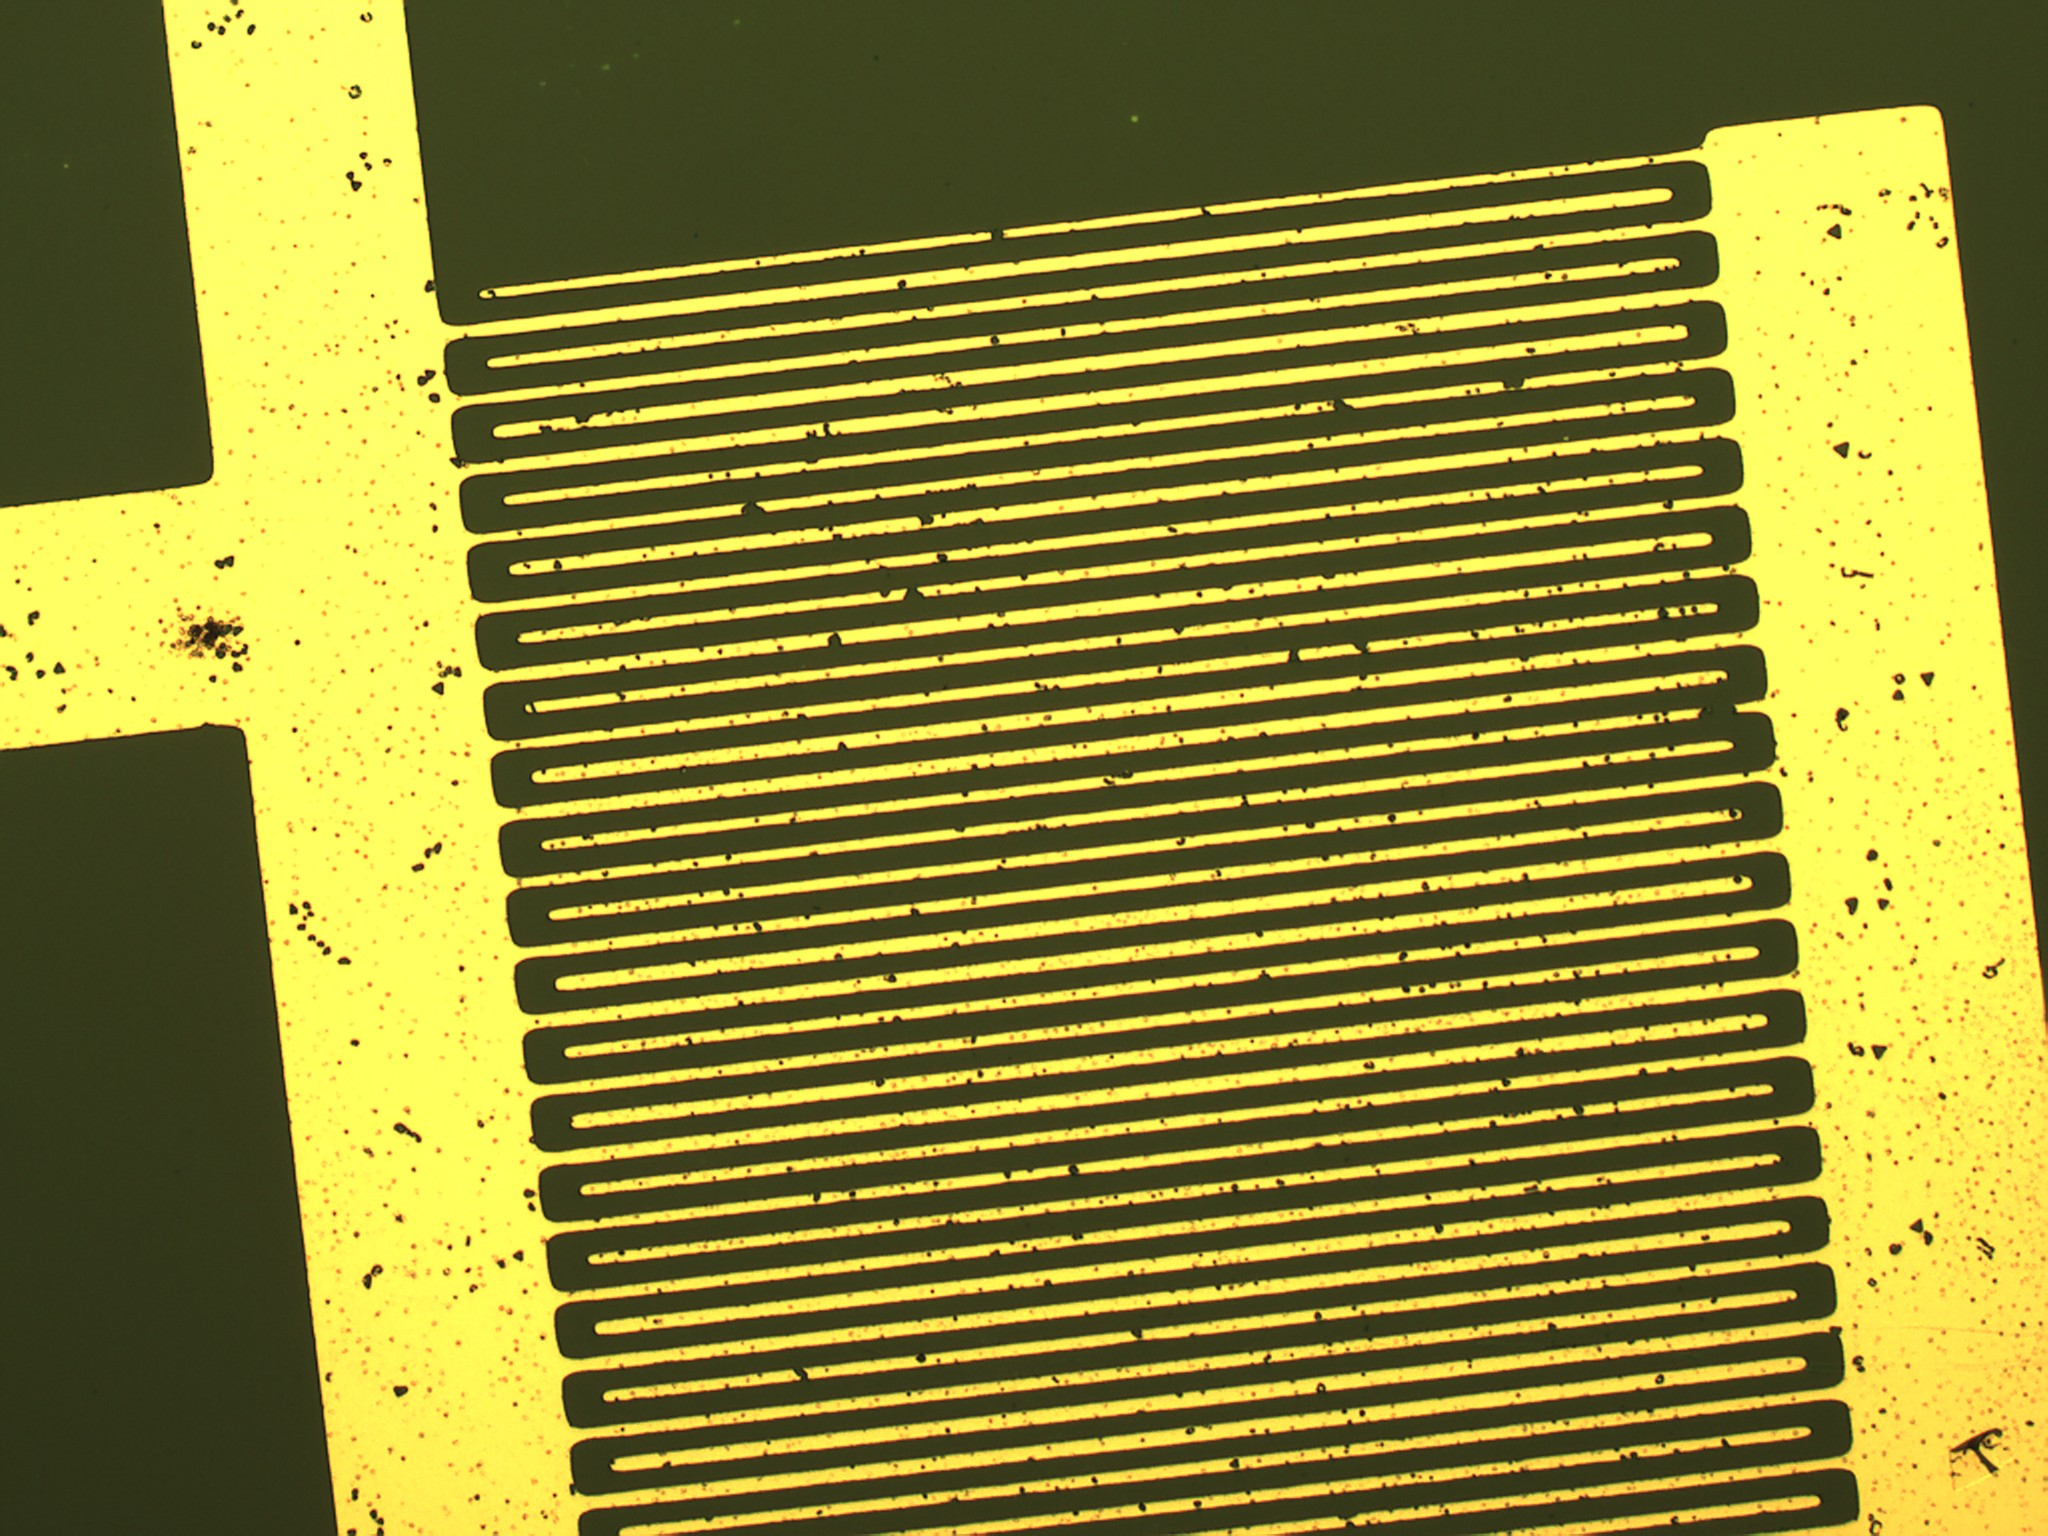
\includegraphics[width=\textwidth]{lithography.jpg}

\end{subfigure}
\begin{subfigure}{0.4\textwidth}
	\caption{}
	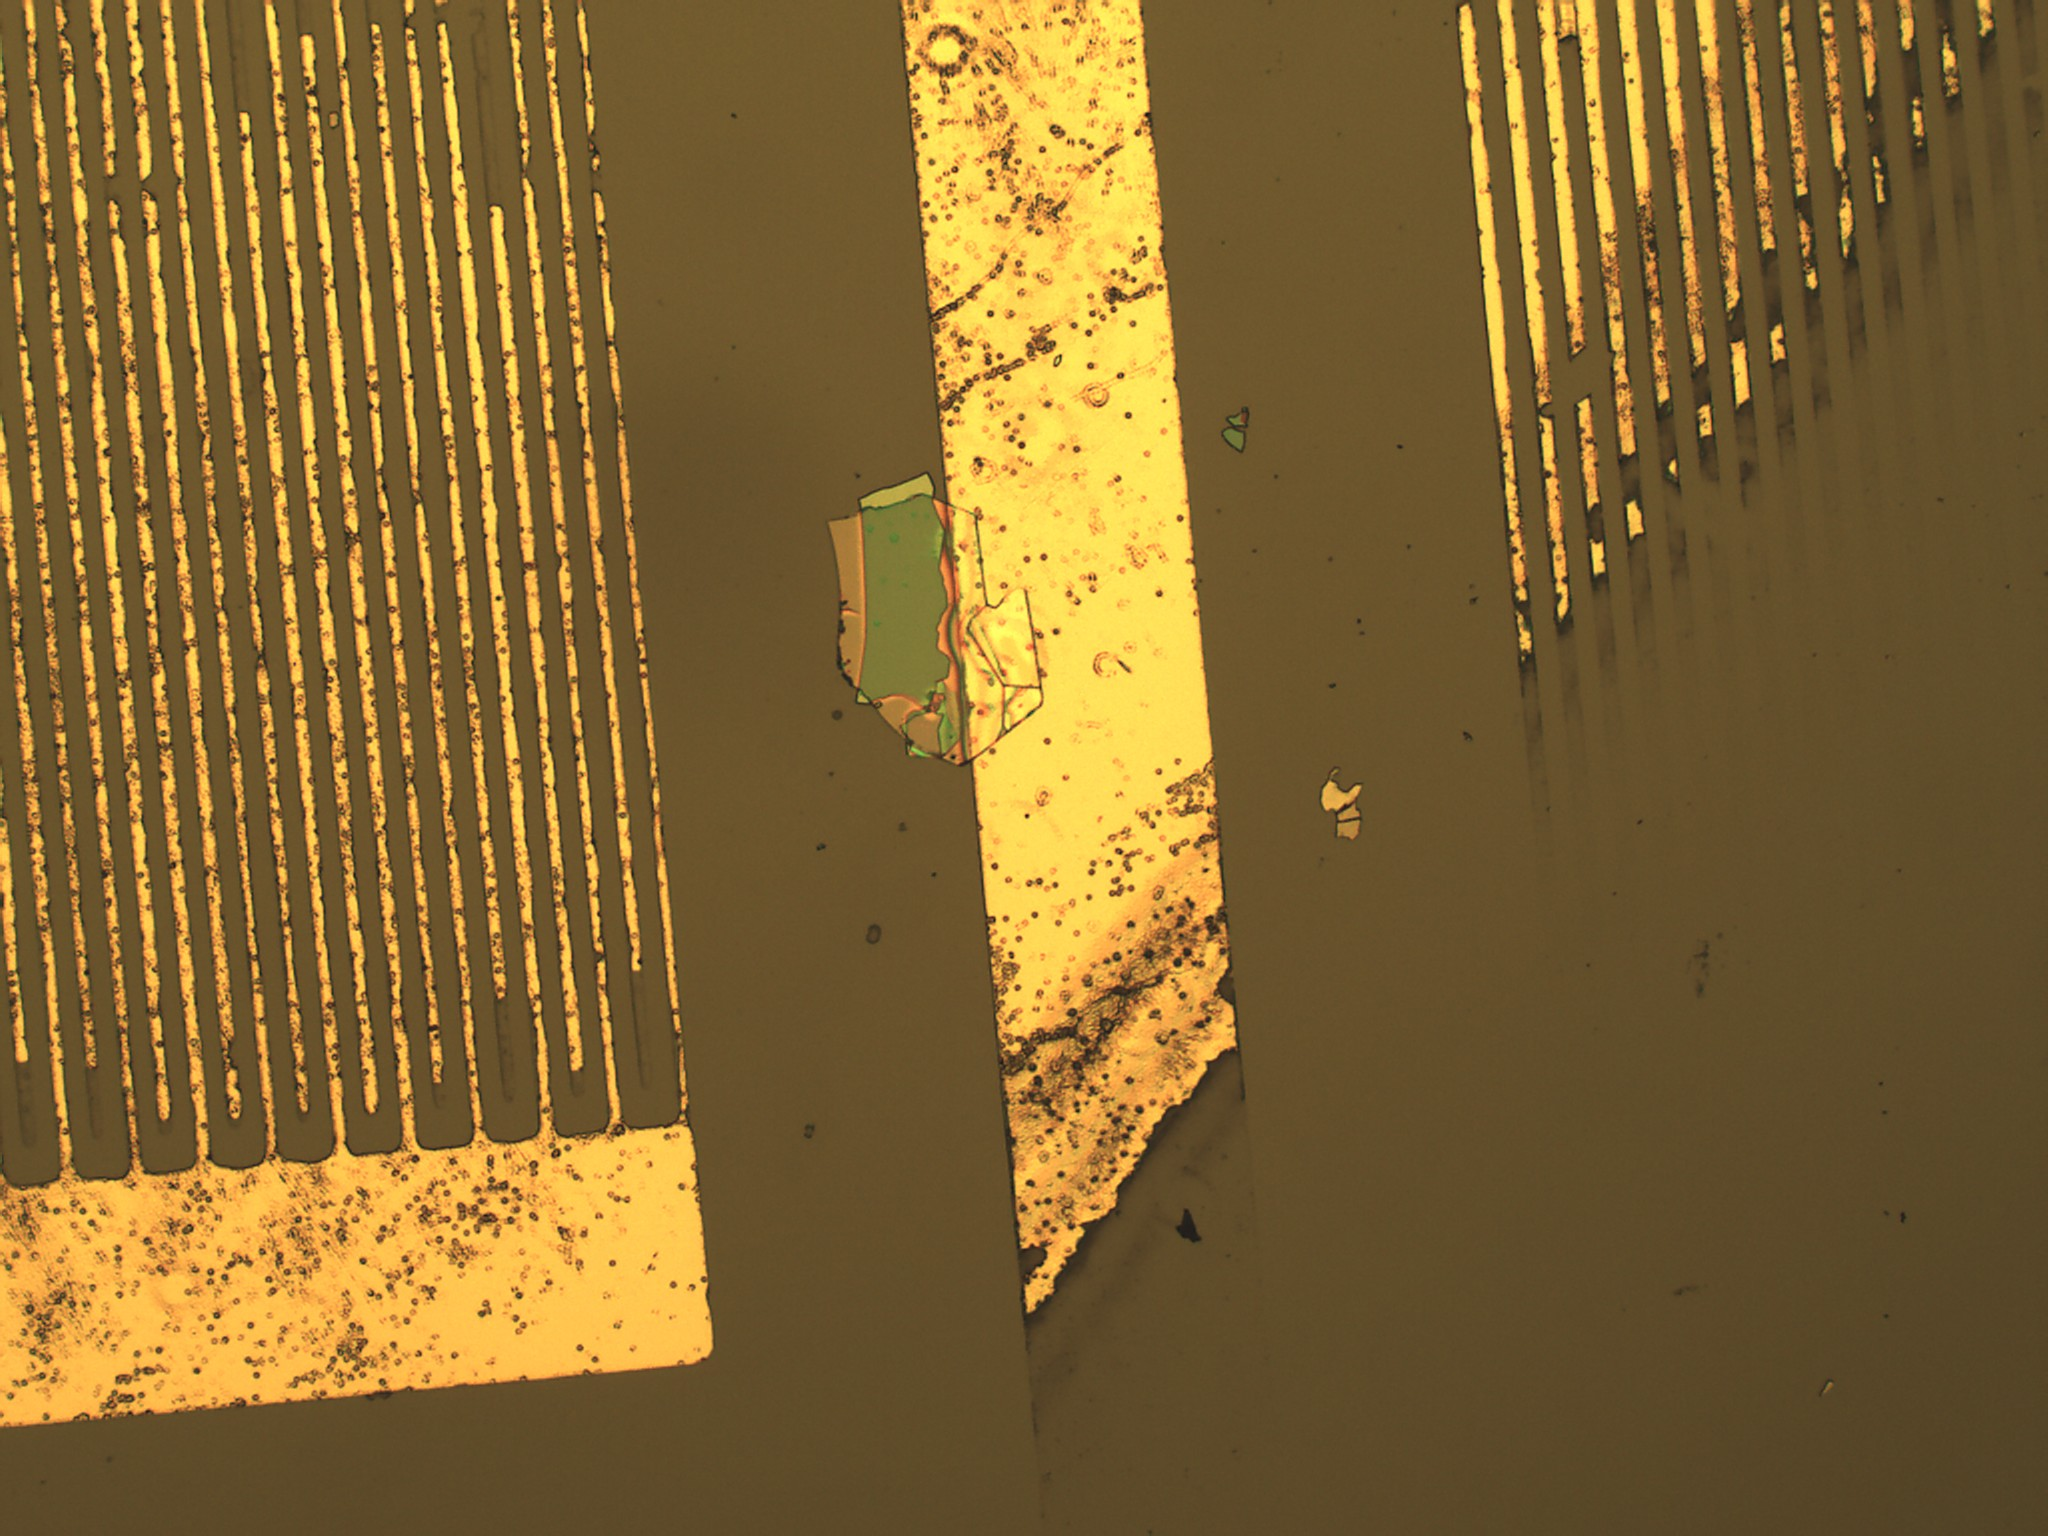
\includegraphics[width=\textwidth]{full_device.jpg}
\end{subfigure}
\caption{\textbf{A} Electrodes are written onto the substrate prior to the assembly of the \hbn-\tmdg heterostructure. A preused chromium mask of an interdigital structure is used for the gold pattern. \textbf{B} As long the heterostructure is dropped in contact with a thick line of the gold pattern, minor defects in the electrode structure do not affect the functionality of the device.}
	\label{pattern}
\end{figure}

In many gated devices, that incorporate \tmd-monolayers, the gate electrodes are actually fabricated directly onto the sample as a last step(Referenzen). While the fabrication of contacts can be more precisely tailored in this way, the big drawback is the exposure of the monolayers to a lot of chemicals like photoresist and developer, that can contaminate the sample and lower its quality. Therefore in this work a more simple approach was chosen. Instead of writing contacts after transfer, contacts are fabricated beforehand. The encapsulated \hbn-\tmd-heterostructure can be contacted by dropping it on the edge of the gold structure.

The gold patterns are created using contact lithography using a chromium mask, deposited on glass. Because the heterostructure can be dropped at any point on the substrate, the precise shape of the gold structure is unimportant. Therefore no new lithographic mask had to be fabricated. Instead a suitable mask was chosen from old preused structures. The downside is, that these masks can deteriorate over time and over many uses, but because of the low requirements for the electrodes all its defects manifest themselves in a purely aesthetic manner and do not affect its functionality.

The process starts with spin coating blabla-photoresist on a \si/\sio wafer. Using the blabla-Maskaligner, the wafer is brought in contact with the mask before exposing it to \textsc{uv}-light for 18 seconds. After that, the pattern is developed using blabla-developer, that washes out the exposed photoresist.

In the next step, the sample is coated in an X-ray evaporation system. First, a 1-5nm film of titanium is deposited on the substrate, that acts as a bonding agent. Subsequently a 50nm film of gold is deposited ontop, that forms the actual top-gate electrode. After removing the sample from the high-vacuum chamber the undevelopped photoresist is removed in the so called ``lift-off''. The substrate is simply bathed in acetone, that desolves the resist below most of the deposited gold and only the structures in the developped areas remain. To speed up the lift-off process, the sample can be placed in an ultrasonic cleaner at a low power.

The resulting structure can be seen in Figure \ref{pattern}. 

\section{Hot pick-up and transfer}

\begin{figure}
	\centering
	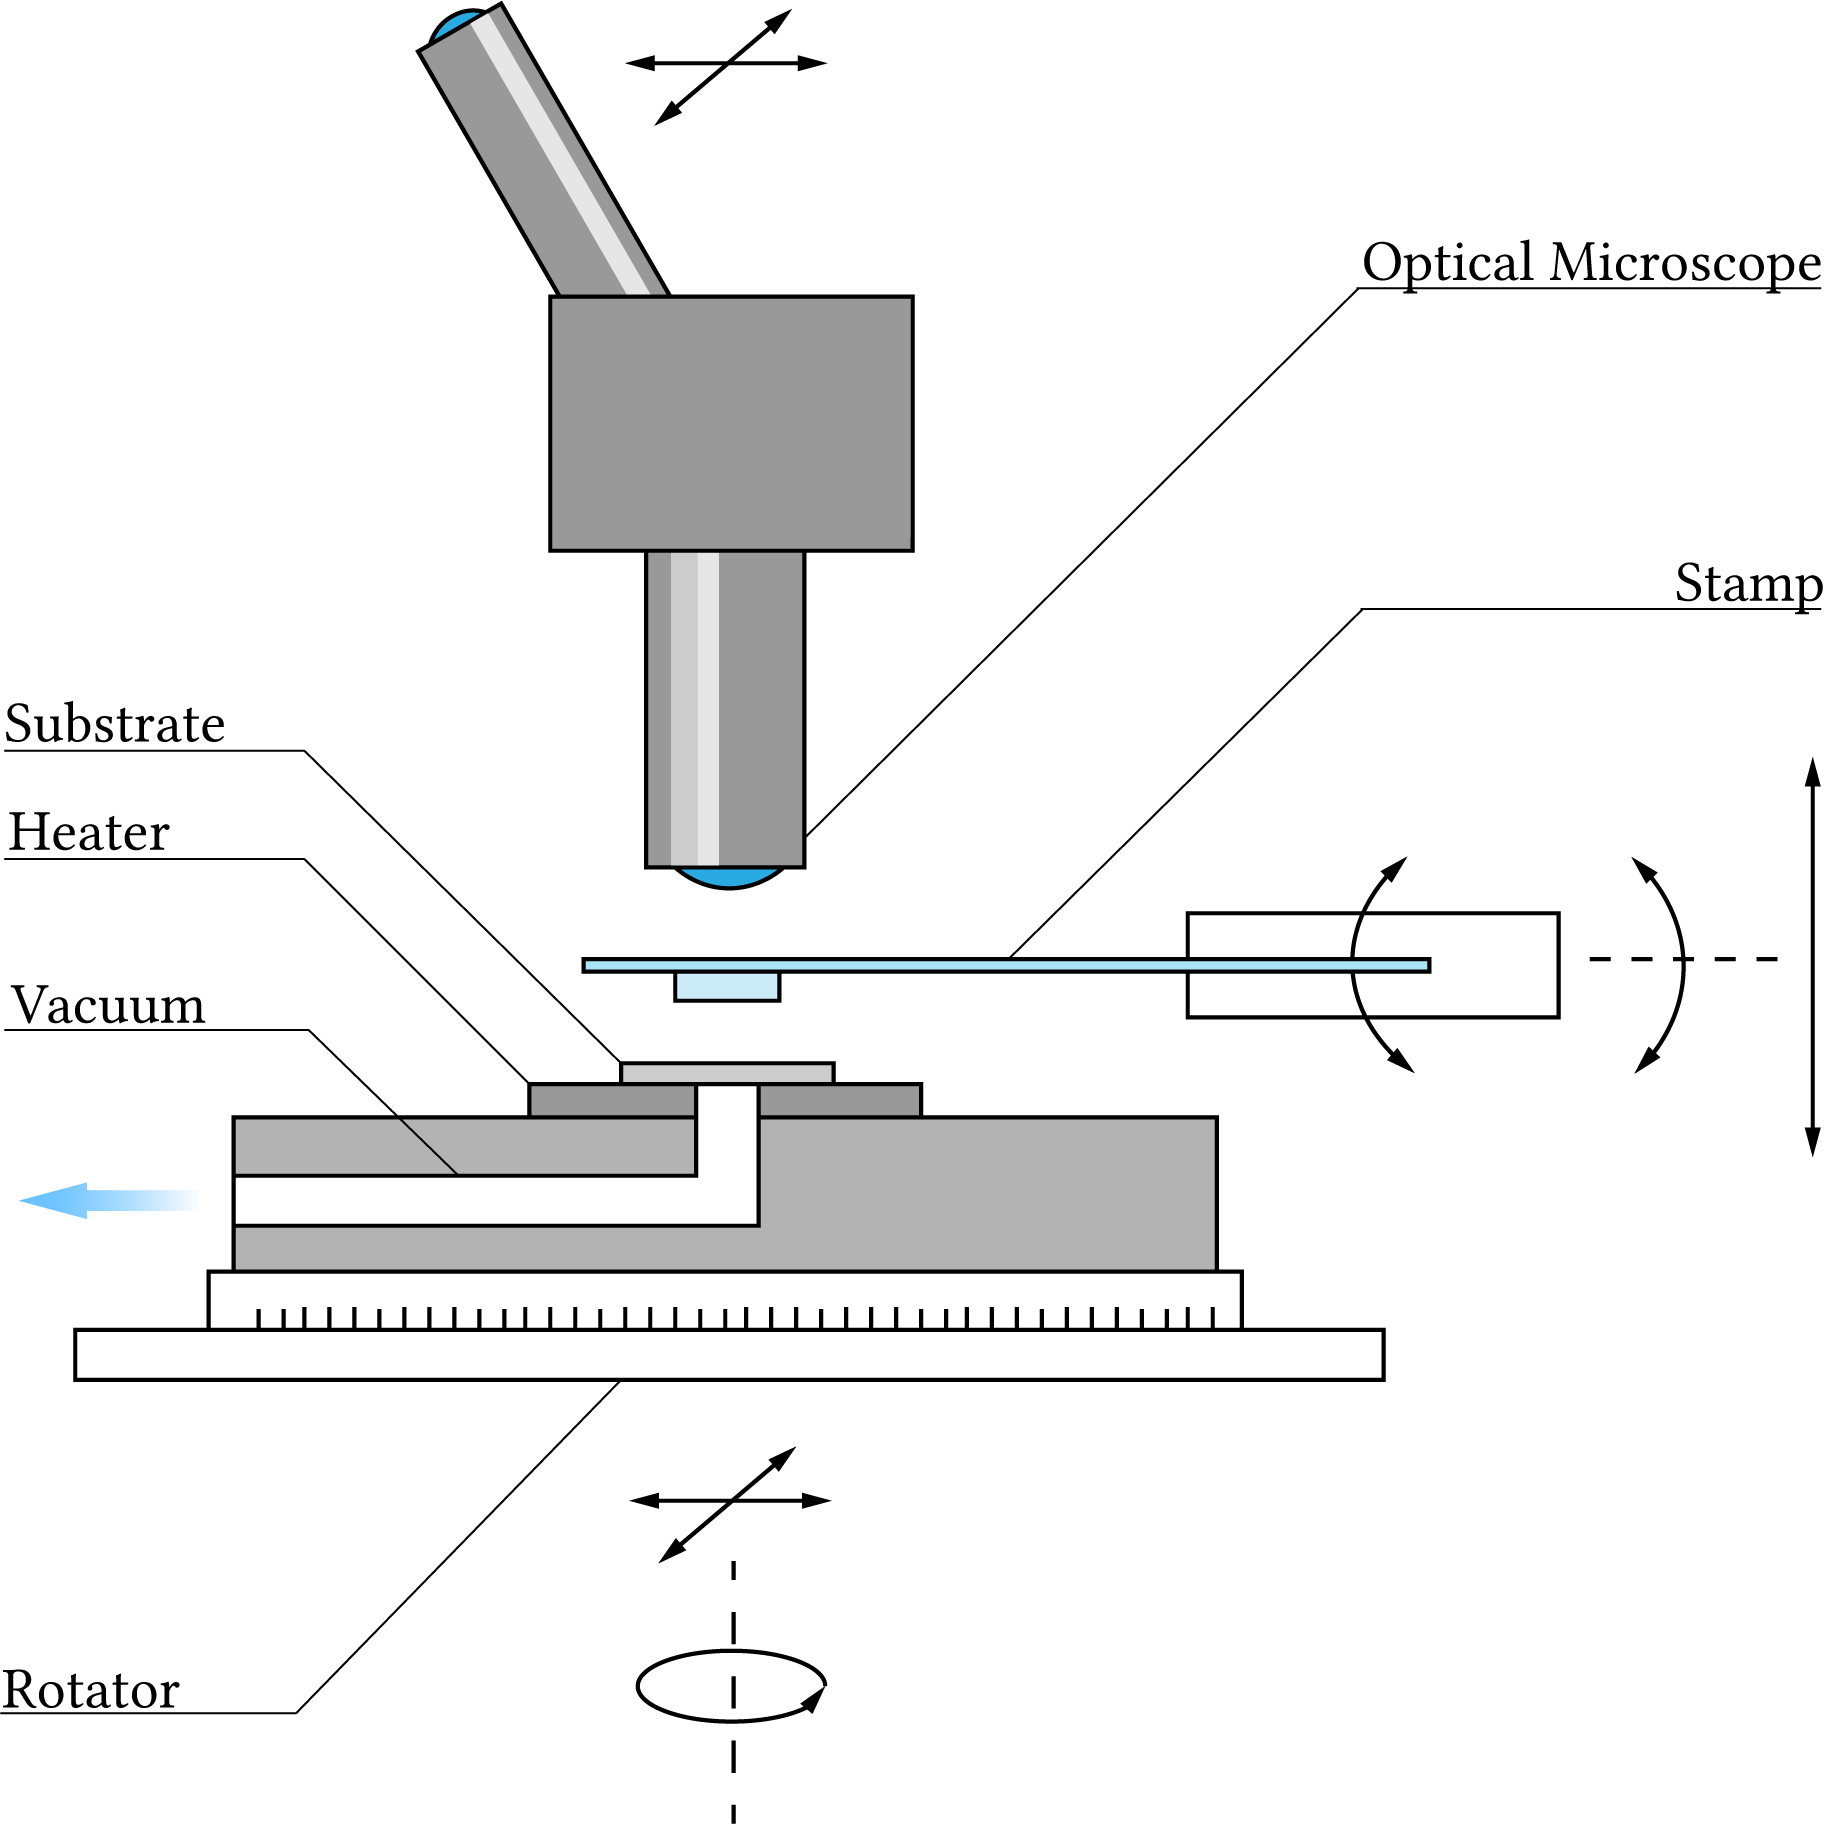
\includegraphics[width=0.7\textwidth]{Stempelaufbau.png}

	\caption{Setup for hot pick-up and stamping. The substrate is placed on a small, round \textbf{ceramic heater} with a 3mm whole in the center(Referenz Thorlabs), that is \textsc{pid}-controlled and can reach temperatures up to 200°C. It is mounted airtight onto the massive sample holder, that is connected to a \textbf{vacuum pump} to hold the \textbf{substrate} in place. It is \textbf{fully rotatable} and can be moved in plane. The \textsc{pdms/ppc} \textbf{stamp} is monted to a z-translator and can be tilted with respecto to both in-plane axes. The \textsc{optical microscope} can also be moved in-plane.}
	\label{stamping-setup}
\end{figure}

The mechanical exfoliation method is popular also for its synergy with dry transfer methods. \textsc{Cvd}-grown \tmd-flakes are grown on suitible substrates and can be transferred to target substrate using a variation of wet methods, that involve powerful solvents or a combination of solvents and polymer films to lift the grown flakes off their initial substrate(Referenz PMMA method etc.). The advantage of the exfoliation method in this regard is that flakes can be put on any substrate directly from the adhesive tape. That led to the invention of ``viscoelastic stamping'', where the \tmd-material is exfoliated on a substrate of viscoelastic polymer called polydimethylsiloxane (\textsc{pdms})(Reference). This so called ``stamp'' could then be brought in contact with the target substrate and peeled off carefully to drop down the flake at a desired condition opening up the possibility of producing carefully designed heterostructures deterministically.

The requirement to sandwitch samples in \hbn opened up the possibility of using the van-der-Walls forces between \hbn and 2D-materials not only to drop down exfoliated layers, flake by flake but to pick up 2D-materials with \hbn-flakes, inreasing the yield as well as ensuring very clean interfaces, free of contaminants of the polymer stamp. 

The method used for this work is called ``hot pick-up and stamping'' (Reference). The stamp used in this process is a block of \textsc{pdms}, mounted on a glass slide with transparent adhesive tape. This block is spin-coated with a polymer polypropylene carbonate (\textsc{ppc}). To make sure, that the polar \textsc{ppc} sticks to the stamp while being heated to high temperatures it is treated in oxygen plasma for at least 20 minutes before the spin coating.

The \tmd-flake is exfoliated on a Si/SiO$_2$ substrate and so are suitible bottom and top \hbn flakes. The primary criteria for finding the right \hbn-flakes is the flattness of its surface, so that the \tmd-flake can be encapsulated between two large terasses without cracks or steps. To allow a fast fabrication process, this flattness is only judged with help of an optical microscope. More sophisticated methods like atomic force microscopy can be used to verify the flattness more accurately, however this not only extends the fabrication process but does not help determining the quality of the top \hbn flake, since its interface is facing down after being exfoliated on the parent substrate.

The goal of the hot pick-up is now to use a hot-plate to control the van-der-Waals forces between \hbn, \tmds and the substrate to ensure adhesion between the parts of the heterostructure as well as to reduce contamination with water molecules from the ambient air.

After all precursors are prepared on Si/SiO$_2$ substrates, the actual pick-up and stamping process can be carried out. The fabrication setup can be seen in (Figure whatever). The first step is the pick-up of the top \hbn flake. At 40°C the van-der-Waals forces between \hbn and \textsc{ppc} are already strong enough to lift the flake off the silicon substrate. In the next step the \hbn is dropped dropped on the \tmd-flake. To make the interface as clean as possible the temperature for this drop is raised to 110°C. This ensures a stronger van-der-Waals force between \hbn and TMD than between TMD and silicon-dioxide but more importantly contamination through droplets of water from the ambient air is minimized above its boiling point and other contaminants are more mobile as well. By slowly pressing the stamp against the substrate, this dirt can leave the interface of the two flakes and fewer blisters form(hotpickuppaper). The stack of TMD and \hbn can then be picked up again following the same procedure that was used for the bare \hbn flake. Afterwards it is dropped down on the bottom \hbn flake. To contact the TMD flake to gold part of it has to remain outside the \hbn encapsulation. This part does not necessarily have to be a monolayer but can also be any form of TMD, that is in contact with it so charges can be transported. The \hbn on the other hand is elastic enough so that thicker material does not affect the encapsulation of mono- or bilayer regions.

The last step is to transfer the whole stack to its final position in contact with the electrodes. This is accomplished by repeating the pick-up process once again and dropping the stack in contact with the gold structure.

Despite the strong plasma treatment of the \textsc{pdms}-stamp in some cases the \textsc{ppc} can peel off during the drop down part of the transfer due to high heat as the polymer becomes ever more liquid. In this case the sample can be carefully treated with acetone, which dissolves the polymer rapidly. The sample subsequently has to be cleaned in isopropanole and blown dry with nitrogen gas. 

\subsection{Annealing}

While the hot pick-up should in theory ensure a \hbn-TMD interface free of contamination, especially contamination due to humidity in the ambient air can remain between the layers and seriously lower the quality of the sample. To remove this pollution, the sample can be annealed(Referenz). During annealing, the sample is placed in an annealing oven. While maintaining a high vacuum of 10$^{-3}$ mbar, the oven heats the sample up to 250°C for around three hours. Other recipes, that use higher or lower temperatures or longer annealing times can work just as well as long as they ensure the complete evaporation ov residual water. 

Different groups report different recipes for this procedure(Referenzen). During the hot pick-up method the \tmd-flakes are never in contact with anything but ambient air and cleanly cleaved \hbn-interfaces. More aggressive recipes, that work at higher temperatures or for longer times to remove also contaminations that arise from the stamp therefore have a limited advantage over milder annealing conditions.